\documentclass[tikz]{standalone}
\tikzset{
  column separations bo/.style={
    /utils/exec=\def\pgfmathcounter{0},
    /utils/temp/.style={
      /utils/exec=\edef\pgfmathcounter{\pgfinteval{\pgfmathcounter+1}},
      /tikz/column \pgfmathcounter/.append style={column sep={{##1},between origins}}},
    /utils/temp/.list={#1}}}
\begin{document}
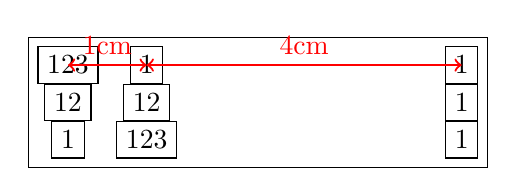
\begin{tikzpicture}
\matrix[
  draw,
  column separations bo={1cm,4cm},
  nodes=draw] {
    \node(a) {123}; & \node (b) {1};   & \node {1}; \\
    \node    {12};  & \node     {12};  & \node {1}; \\
    \node    {1};   & \node     {123}; & \node {1}; \\
  };
\path [<->,red,thick,above] (a.center) edge node {1cm} ++(right:1cm)
                            (b.center) edge node {4cm} ++(right:4cm);
\end{tikzpicture}
\end{document}